\section{Vorbereitungsfragen}
\subsection{Photovoltaik-Inselanlage}
\subsubsection{Geben Sie vier Konzepte von PV-Inselanlagen mit je einem Einsatzbeispiel an}
Die möglichen Konzepte für eine PV-Inselanlage unterscheiden sich innerhalb der verwendeten
Komponenten und entsprechend auch durch die möglichen Verbraucher und die Verschaltung.\\
Das einfachste der vier Konzepte ist das direkte Verschalten der PV-Anlage mit
DC-Verbrauchern, hierbei kann es sich z.B. um ein Heizungssystem für ein Schwimmbecken handeln.\\
Das zweite System wird durch eine Batterie ergänzt welche zwischen die PV-Anlage und die Verbraucher geschaltet ist.
Mögliche Anwendungen sind einfache DC-Systeme, welche allerdings auch außerhalb der Sonnenstunden
funktionieren müssen und dementsprechend einen Puffer benötigen. Ein Beispiel wäre hier ein solarversorgter Snackautomat.\\
Das komplexeste System welches weiterhin für DC-Verbraucher gedacht ist, wird neben den Komponenten des zweiten Systems
um einen Laderegler ergänzt welcher vor die Batterie geschaltet wird. Solche Systeme werden häufig in
Wohnmobilen oder Wohnwägen verwendet, welche mit DC-Verbrauchern ausgestattet sind.\\
Um AC-Verbraucher nutzen zu können muss zusätzlich zu System 3 ein Umrichter vor die Verbraucher geschaltet werden, um diese
korrekt versorgen zu können. Diese Systeme können dann Einfamilienhäuser, Forschungsstationen oder abgelegene Dörfer versorgen und ein Netz etablieren.\\ 
\subsubsection{Die Anlagenkomponenten sollen im Inselsystem auf ihre Funktionsfähigkeit hin geprüft werden. Was messen Sie in welcher Reihenfolge?}
Gemessen werden an allen Eingängen und Ausgängen der Geräte sowohl der Strom als auch die Spannung.
Beginnend mit dem Ausgang der PV-Anlage, wird dann entlang der Erzeugungslinie geprüft.
So folgt die Prüfung des Ladereglers. Anschließend wird das Batteriesystem geprüft und abschließend der 
Umrichter.\\


\subsection{Laderregler}
\subsubsection{Welche Voraussetzungen müssen Anlagen mit Akku ohne Laderegler haben? Wann wird ein Laderegler notwendig?}
Inselnetzanlagen müssen in der Lage sein, die Ladung des Akkus und die Stromversorgung des angeschlossenen Verbrauchers zu gewährleisten. Dementsprechend müssen die einzelnen Bauteile aufeinander ausgelegt werden, um eine Beschädigung der Komponenten zu vermeiden. Ein Laderegler wird benötigt, sobald die Leerlaufspannung der Module die maximale Ladespannung der Batterie überschreitet, eine spannungsunabhängige Schaltung umgesetzt werden soll (bei größeren Anlagen) oder keine konstanten Wetterbedingungen garantiert werden können. Ein Laderegler sorgt dafür die Batterie vor Tiefenentladung und Überladung zu schützen. In Kombination mit einem MPP-Tracker kann ein Laderegler auch den Energieertrag erhöhen. 
\subsubsection{Geben Sie Verfahren zur Laderegelung in PV-Inselanlagen an und erläutern Sie deren Funktionsprinzip! Unter welchen Bedingungen ist welches Verfahren von Vorteil? (Beachten Sie auch den Kostenaspekt!)}
Es wird in drei unterschiedliche Arten von Ladereglern (LR) unterschieden:
\begin{itemize}
\begin{figure}[!h]
		\centering
		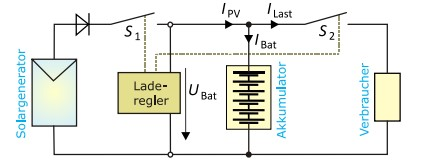
\includegraphics[width=0.7\textwidth]{Abbildungen/Serienladeregler}
		\caption{Photovoltaik-Batteriesystem mit einem Serienladeregler  }
		\label{fig:Serienladeregler}
\end{figure}
\item In Serienladereglern (auch Längsregler) (\autoref{fig:Serienladeregler}) werden Leistungshalbleiter als Schalter verwendet um den Stromfluss zu unterbrechen. Das hat zur Folge, dass beim Laden des Akkus immer Durchlassverluste entstehen. Serienladeregler sind die preiswertesten LR und können auch für nicht kurzschlussfeste Verbraucher genutzt werden. 

\begin{figure}[!h]
		\centering
		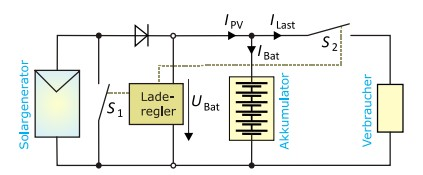
\includegraphics[width=0.7\textwidth]{Abbildungen/Shuntladeregler}
		\caption{Photovoltaik-Batteriesystem mit einem Shuntladeregler}
		\label{fig:Shuntladeregler}
\end{figure}

\item Shuntregler (auch Parallelregler) (\autoref{fig:Shuntladeregler}) sind am weitesten verbreitet. Diese schalten bei vollgeladenem Akku den Solargenerator kurz. Dieser Kurzschluss stellt im regulären Betrieb kein Problem dar kann aber bei Abschattungen zu extremen Belastungen einzelner Zellen führen.

\item MPP-Laderegler können auch bei wechselnden Wetterbedingungen beste Ladeleistungen erreichen. Nachteilig sind allerdings die hohen Anschaffungskosten.

\end{itemize}
\subsubsection{Es soll eine defekte Batterie des Batteriesystems aus der Anlage gewechselt werden. Geben Sie die Reihenfolge Ihres Vorgehens schrittweise an.}
Das Wechseln der Batterie erfolgt in 7 einzelnen Schritten. Als erste sollte die Betriebsanleitung gelesen und danach die Last abgeschaltet und vom System getrennt werden. Darauffolgend muss sowohl der PV-Generator als auch die Batterie vom Laderegler getrennt werden. Nun kann die neue Batterie und danach der PV-Generator an den Laderegler angeschlossen werden. Als letztes wird die Last wieder angeschaltet.

\subsection{Batteriesysteme}
\subsubsection{Welche Batterie-Typen werden in PV-Anlagen häufig eingesetzt? Nennen Sie Vor-und Nachteile! Was ist bei deren Laderegelung zu beachten?}
Die beiden am häufigsten verwendeten Akkumulatoren sind Blei- und Lithium-Ionen-Akkus.
Blei Akkus haben zum Vorteil, dass sie schon sehr lange beispielsweise für Kraftfahrzeuge in der Benutzung sind und so sehr weit optimiert werden konnten. Außerdem sind die Speicher preiswert und leicht zu erwerben. Nachteilig sind sowohl die geringe Energiedichte (im Vergleich mit Lithium Akkus) als auch die Selbstentladung von ca. 10\% pro Monat (bei 25°C). Um eine Tiefenentladung zu vermeiden, müssen Bleiakkumulatoren deshalb regelmäßig nachgeladen werden. Dazukommend darf der Akku nicht mit zu hoher Spannung geladen werden um Gasung zu vermeiden. Deshalb muss bei der Wahl eines Batterieraums auf eine gute Durchlüftung geachtet werden.\\\\
Lithium-Ionen-Akkus zeichnen sich durch ihre hohe Energiedichte und geringe Selbstentladerate aus. Beachtet werden muss allerdings der höhere Preis und die zeitweilig geringe Verfügbarkeit auf Grund der hohen Nachfrage. Ein weiterer Nachteil ist die Empfindlichkeit der Batteriezellen, weshalb diese mit einem elektronischem Batteriemanagementsystem überwacht und geschützt werden müssen.\\\\
Bei der Ladereglung von Batteriesystemen ist es besonders wichtig auf die Ladeströme und Spannungen, die Batterieräume als auch auf die Empfindlichkeit der Batteriezellen zu achten, um Beschädigungen des Systems zu vermeiden.

\subsubsection{Welche Anforderungen werden an einen Batterieraum gestellt?}
Ein Batterieraum sollte trocken, gut belüftet, mit einem Rauchmelder ausgestattet und gleichmäßig im zulässigen Temperaturbereich temperiert sein.
\subsubsection{Geben Sie die häufig eingesetzten Systemspannungen an! Was ist bei Gleichspannungsverbrauchern (insbesondere bei niedriger Spannung) im Vergleich zu Wechselstromverbrauchern zu beachten?}
Häufige Systemspannungen sind 12 V, 24V, 48V, und 72V.
Bei DC-Verbrauchern kann es zu hohen Strömen kommen weshalb große Kabelquerschnitte vorteilhafter sind.


\subsection{Wechselrichter in PV-Inselanlagen}
\subsubsection{Nach welchen Kriterien erfolgt die Auswahl eines Insel-Wechselrichters?}
\begin{itemize}
    \item Die Leistung des Umrichters muss an die Leistungs anforderungen des Insel-Netzes angepasst werden.
    \item Die Signalqualität der Spannung muss auch unter Last in den erforderten grenzen der Verbraucher bleiben.
    \item Der Wirkungsgradbereich muss nach dem Lastverhalten des Inselnetzes ausgelegt werden.
    \item Der Umrichter muss die gleiche Phasen-Anzahl besitzen, wie das System benötigt.
\end{itemize}
\subsubsection{Welche Insel-Wechselrichter-Typen können zum Einsatz kommen (Kosten beachten)?}
Mögliche Umrichter Typen:
\begin{itemize}
    \item mit oder ohne inneren Trafo
    \item 3 Level oder Multi Level
    \item 1 oder 3 Phasig
    \item Single- oder Multistring
\end{itemize} 
\subsubsection{Woran erkennen Sie während des Betriebes einen 'schlechten' Wechselrichter? (niedriger Wirkungsgrad)?}

\begin{itemize}
    \item Die Qualität der Spannung ist durch Oberschwingungen und Verzerrungen unzureichend.
    \item Der Umrichter produziert zu große mengen an Wärme im Nennlast betrieb.
    \item Der momentan Wirkungsgrad des Wechselrichters kann mit hilfe von \autoref{eq:230430_WR-Wirkungsgrad} bestimmt werden.
    \item Wenn der Wirkungsgrad bei Nennleistung deutlich unter einem wert von 90\% liegt, kann der Umrichter als 'schlecht' bezeichnet werden.
\end{itemize}

\begin{equation}
    \eta_{WR} = \frac{P_{WR,Ein}}{P_{WR,Aus}}
    \label{eq:230430_WR-Wirkungsgrad}
\end{equation}

\subsubsection{Welche Anforderungen an den Einbauort des Wechselrichters müssen gewährleistet sein?}
\begin{itemize}
    \item Der Einbauort muss vor Witterung schützen.
    \item Der Umrichter muss gut belüftet sein.
    \item Die Umgebungstemperatur des Umrichters, darf zu keiner zeit auhßerhalb seines angegebenen Temperaturbereichs liegen.
    \item Die Umrichter sollten für Wartungszwecke leicht zugänglich sein.
    \item Ein brand sollte möglichst schnell erkannt werden, durch z.B. Brandmelder und sollte keine anderen komponenten beeinflussen durch genügend Abstand oder abschirmung.
\end{itemize}
\subsubsection{Unter welchen Umständen muss am WR einer PV-Inselanlage sofortige Lastabschaltung erfolgen?}
Bei jedweder gefahr entdeckung für die verbraucher:
\begin{itemize}
    \item überspannungen durch z.B. Blitzeinschlag
    \item Kurzschlüsse durch z.B. Hochwasser
    \item Bei Feuer am Umrichter.
\end{itemize}
\subsubsection{Wie wirkt sich die benötigte Blindleistung auf die Dimensionierung des Wechselrichters aus?}
Durch zusätzlich benötigte Blindleistung muss der Umrichter nicht auf die Leistung des PV-Generators ausgelegt werden, sondern auf die scheinleistung, welches er ins netz geben muss.
Diese wird also zusätzlich innerhalb des Umrichters generiert, führt aber zu größeren Leistungflüssen.\cite{SMA_Q-Auslegung}
\subsubsection{Ein PC (einschließlich Peripherie) benötigt 120 W. Der Inselwechselrichter der unter 3. beschriebenen Anlage schaltet wegen Batterieerschöpfung nach 2 Tagen Betriebsdauer ab. Welche Möglichkeit des Dauerbetriebs der Anlage schlagen Sie vor. Begründen Sie die Realisierbarkeit.}
Es wird ein Umrichter benötigt, welcher sowohl Spannungsgeregelt als auch Stromgereglet betrieben werden kann, um zwischen Inselbetrieb und Netzbetrieb wechseln zu können.
\subsection{Einstrahlung und Umgebungsbedingungen}
\subsubsection{Welche aus verschiedenen physikalischen Prinzipien resultierenden Messverfahren zur Erfassung der Globalstrahlung kennen Sie?}
Es gibt 2 Physikalische Effekte, welche konventionell zu messung der Globalstrahlung verwendet werden. 
Der Photo-Effekt, welcher in Pyranomatern mit Halbleitersensoren verwendet wird. 
Dieser Basiert auf dem selben Prinzip wie eine Photovoltaikzelle und setzt die Einstrahlung in Proportion mit dem Strom.
Außerdem kann der Seebeck-Effejt verwendet werden, welcher in thermischen Pyranometern verwendet wird.
Hierbei wird eine von zwei miteinander verbundenen metallplatten durch die Bestrahlung aufgeheizt. 
Der Seebeck-Effekt besagt, dass durch eine Temperaturdifferenz zwischen 2 Leitermaterialien eine elektrische Spannung entsteht.\cite{Wiki-Seebeck}
Dies hat den Vorteil, dass ein viel größerer Teil des Spektrums gemessen wird.

\subsubsection{Welchen Einfluss haben diffuse und direkte Sonnenstrahlung auf die Leistung des PV-Generators?}
Der PV-Generaotr kan problemlos sowohl direkter als auch difuser Bestrahlung Leistung entnehmen. 
Jedoch hat die Difuse Einstrahlung eine geringere spezifische Leistung, da sie mehrweg durch die Atmosphäre zurückgeleht hat und somit einige Wellenlängen durch Absorptionsbänder herausgefiltert wurden.
\subsubsection{Wovon hängt die Modultemperatur ab und welchen Einfluss hat sie?}
Die Modultemperatue wird durch mehrere Fakotern beeinflusst.
\begin{itemize}
    \item Die Umgebungstemperatur
    \item Die Bestrahlungsstärke
    \item Die Einbauart (Hinterlüftet, aktive Kühlung etc.)
\end{itemize}
Hierbei ist zu beachten, dass nicht alle Wellenlängen des Sonnenlichts in einem Modul in Wärme umgewandelt werden, nur welche mehr Energie als die Bandlücke besitzen.
Diese erzeugen zwar auch ein Elektron-Loch-Paar, Generieren aber durch die übereregung Wärme innerhalb des Halbleiters.
Die Modul Temperatur hat direkten einfluss auf die Leistung des PV-Moduls.
Bei steigender Temperatur sinkt die Modulspannung deutlich und der Modulstrom steigt minimal.
